\section{Exercise 1 - Contiguous allocation}

Consider a system with physical memory of 512MB, in which a management scheme with (contiguous) variable partitions is used with a minimum memory allocation unit of 64B (i.e. the memory space is allocated in multiples of 64 bytes). 
The first 128MB of memory are permanently allocated to the Operating System.

The process table contains, for each active process, the starting address (ADDR) and the size (SIZE) of the relative partition in memory. The memory is allocated with the Worst-Fit strategy. Free partitions are managed through a linked list sorted by decreasing size, in which each node represents a free partition; the nodes of the list consist of two fields: (pointer to the next partition, and size of the partition, both represented on 4 bytes, size, and addresses represented in Byte, with the value 0 used as a null pointer) and are stored in the first bytes of the partition which represent.

Suppose that at a given instant, the process table and the pointer to the first free partition contain the information shown in Figure \ref{fig:cont1}. Represent the changes to the partitions in memory, the process table, and the Free List, following the activation of 2 new processes, P12 and P13, which require respectively 25MB and 150MB of memory, followed by the termination of the P11 process.

\begin{figure}[hbt]
  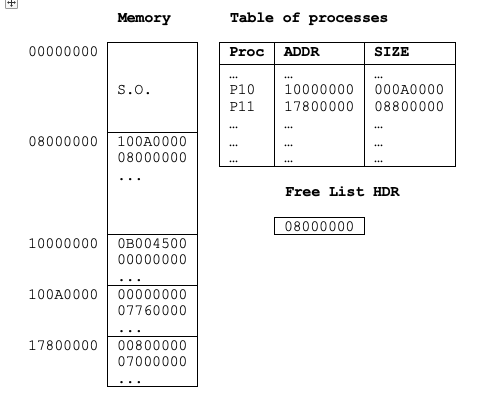
\includegraphics[width=0.8\textwidth]{images/contiguosallocation1.png}
  \caption{Initial condition}
  \label{fig:cont1}
\end{figure}

\subsection{Solution}

Here is the initial setup, which highlights pointers and partition size in memory.

Note that partitions in the free list contain, in their header, size and pointer to the next item in the list. For the allocated partitions, the information contained may be different (as information relating to the processes has been loaded into the partitions).


\begin{figure}[!hbt]
  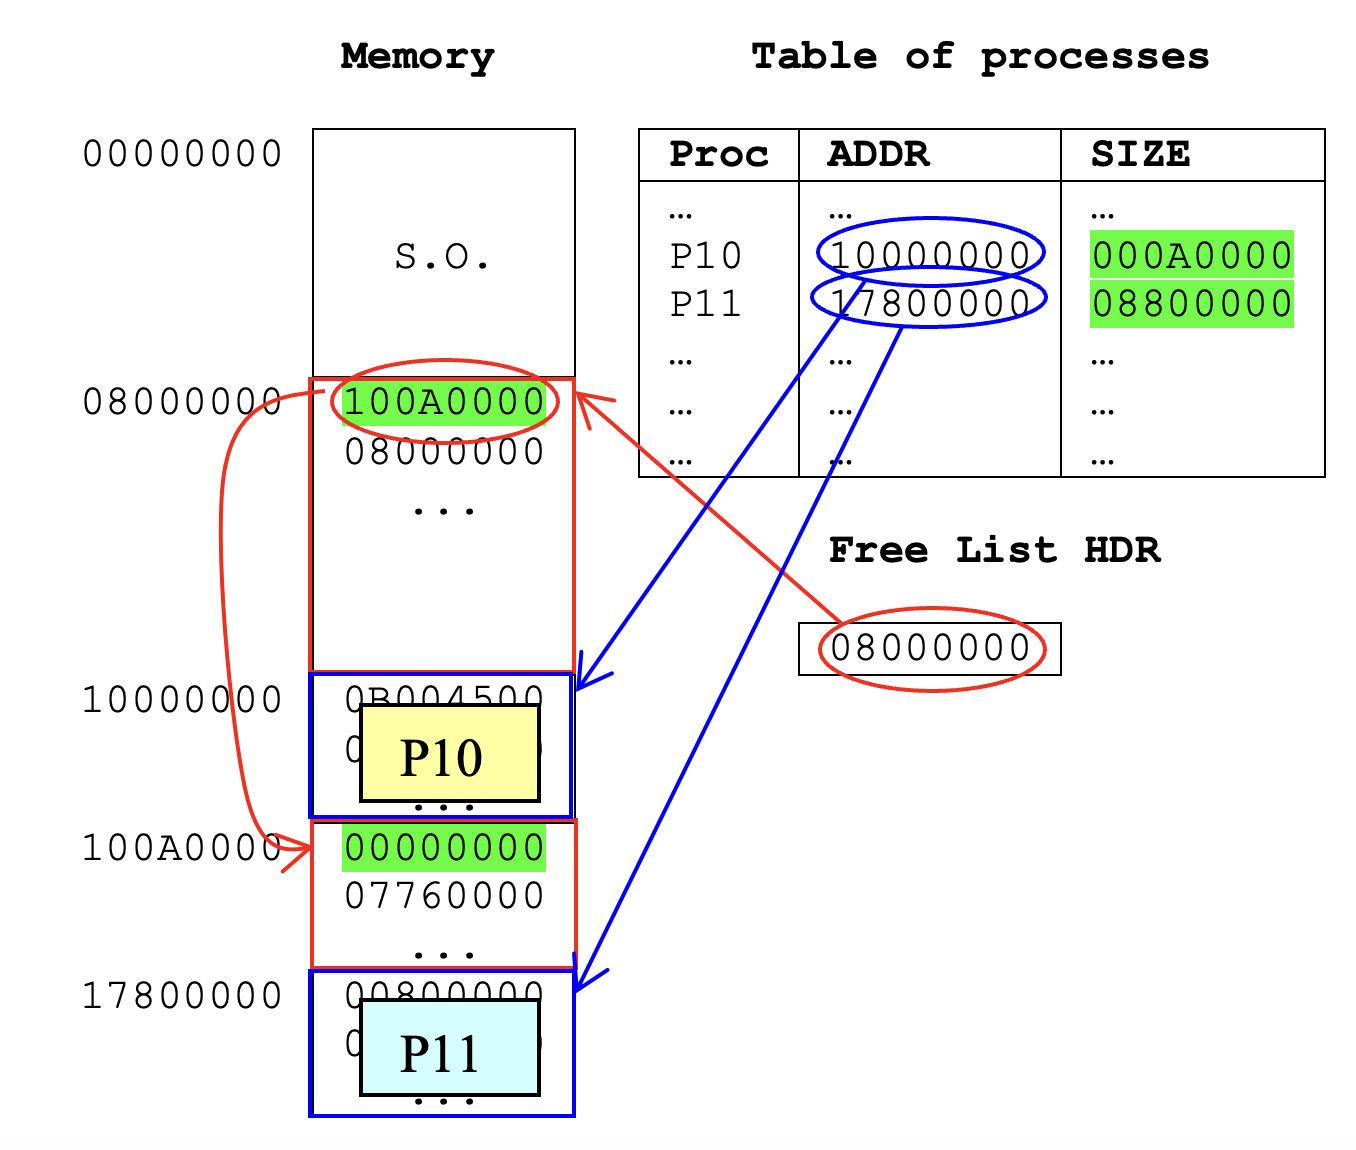
\includegraphics[width=0.8\textwidth]{images/ex01_initial.png}
  \caption{Initial configuration}
  \label{fig:cont1}
\end{figure}

\textbf{In a more compact form, the initial configuration can be represented as follows}

The memory is divided into 5 partitions. The first is allocated to the Operating System, of the remaining 4 partitions, 2 are allocated to processes P10 and P11, and 2 are in the free list. For partitions in the free list, the first 8 Bytes contain the partition size and a pointer to the next. For allocated partitions, the information contained can be of another type.

It is recommended to keep addresses and sizes in hexadecimal. The list of initial partitions, with starting address and size, is:

\begin{verbatim}
hexadecimal
(00000000,08000000), (08000000,08000000), 
(10000000,000A0000), (100A00000,07760000),
(17800000,08800000)
\end{verbatim}


The initial partitions are:

\begin{verbatim}
Free list: (08000000,08000000), (100A0000,07760000)
P10: (10000000,000A0000)
P11: (17800000,08800000)
\end{verbatim}

\textbf{P12 allocation.} 

You need 25MB (in hex 19MB = 01900000 B), which are allocated from the first partition in the free list, from which a free partition remains (of 08000000 B - 01900000 B = 06700000 B). The new free partition goes to the bottom of the free list as it is smaller than the other free partition. Only the variations are shown.

Free list: (100A0000,07760000), (09900000,06700000)
P12: (08000000,01900000)

\textbf{P13 allocation.}  

You need 150MB (in hex 96MB = 09600000 B). None of the partitions are large enough. Various solutions are possible, such as de-fragmentation (by relocation of processes), and swap-out of P10 or P11. The simplest solution is represented: swap-out of P10, which allows you to generate a single free contiguous partition of size 0DF00000 B (given by the sum 06700000 + 000A0000 + 07760000), in which the new partition for P13 is allocated.

\begin{verbatim}
Free list: (12F000000,04900000)
P13: (09900000,09600000) 
\end{verbatim}


\textbf{P11 termination.}

The partition allocated to P11 is freed, increasing the size of the only block in the free list.

\begin{verbatim}
Free list: (12F000000,0D100000)
\end{verbatim}

At this point, you could swap in P10 ...

\section{Exercise 2 - Paging}

Consider a virtual memory system with paging, in which the Bytes are addressed. The system has a TLB (Translation Look-aside Buffer), on which a "hit ratio" of 99\% is experimentally measured. The page table ("page-table") is created with a two-level scheme, in which a 32-bit logical address is divided (from MSB to LSB) into 3 parts: p1, p2, d, respectively of 10-bit, 11-bit, and 11-bit. No additional data structures (such as hash tables or inverted page tables) are used to speed up access.

\begin{itemize}
\item Tell us what is meant by "hit ratio"
\item	Illustrate the layout of the page table and its overall size for a P1 process having a virtual address space of 100MB
\item Calculate external and internal fragmentation for process P1 (see the previous point).
\item Assuming that the RAM memory has an access time of 300 ns, calculate the effective access time (EAT) for the proposed case (hit ratio = 99\%)
\end{itemize}


\subsection{Solution}

The percentage of times a particular page number is found in the TLB is called the hit ratio. 

Note that 100 MByte < 128 MByte = $2^27$ Byte and that pages and frames have a size of 2Kbyte = $2^{11}$ Byte (obtained from d: 11 bit). 

Assuming that each entry in the page tables uses 32 bits (4 Byte), a second-level page table will have $2^{11}$ cells (11 from p2) and size $2^{11}$ * 4 Byte, while a first level page table will have 25 cells (only 5 bits out of 10 of p1) and size of $2^5$ * 4 Byte are needed. 

External fragmentation is 0 by definition. 

The internal fragmentation for a generic process is:
\begin{itemize}
 \item worst case: 2 Kbytes - 1 byte
 \item average case: 1 Kbyte (half of a page)
\end{itemize}

For P1, the internal fragmentation is 0 because the virtual space is a multiple of 2Kbyte.

The	EAT = (0.99 * 300 + 0.01 * 3 * 300) ns = 1.02 * 300ns = 306 ns

\textbf{ATTENTION}: in the case of TLB MISS, there are 3 accesses, not 2 (the page table is on two levels, therefore 2 accesses for the PT plus one for the desired access in RAM)

\section{Exercise 3 - Paging}

Describe the advantages and disadvantages of an inverted page table (IPT) compared to a standard (possibly hierarchical) page table. 

Consider a process having a virtual addressing space of 32 GB, equipped with 8GB of RAM, on a 64-bit architecture (in which the Byte is addressed), with the management of paged memory (1KB pages/frames). You want to compare a standard page table-based solution (one table for each process) and an IPT-based solution. 

Calculate the page table size (at one level only) for the process and the IPT. Let's assume that the pid of a process can be represented on 16 bits. Use 32 bits for page and/or frame indexes. Finally, using the proposed IPT (32 bits for a page/frame index), what is the maximum possible size for the virtual address space of a process?

\subsection{Solution}

Advantages:
\begin{itemize}
\item Memory savings: the table has the size of the physical RAM instead of the virtual address space
\item There is a single table for all processes (each frame is associated with a single process)
\end{itemize}

Disadvantages
\begin{itemize}
\item The real disadvantage is the slowness, you have to search for a page rather than access it directly. For this reason, IPTs are usually associated with hash tables.
\end{itemize}

For size calculations, any validity/modification bits are ignored.

\textbf{Standard Page Table:}

N pages = 32GB / 1KB = 32M (corresponds to the number of frame indexes in the page table)

 Page Table = 32M * 4B = 128MB

\textbf{IPT}

The table, unique for all processes, has a fixed size, as it contains a page index for each frame in RAM (consider, for simplicity, managing all the RAM, including the one assigned to the operating system). Each line of the IPT contains a page index (4B) and the process pid (2B)

N frames = 8GB / 1KB = 8M

IPT = 8M * (4B + 2B) = 48MB

\textbf{Virtual address space}

The maximum number of virtual pages of a process is limited by the size of the page indexes (32 bits): this number is, therefore, 4G. Since each page is 1KB, the virtual address space has a maximum size of 4G * 1KB = 4TB.


\section{Exercise 4 - Page replacement}

Consider the following sequence of references in memory in the case of a 1000-word program: 261, 409, 985, 311, 584, 746, 632, 323, 470, 915, 858.

Determine the string of page references, assuming their size is 200 words. Use a second-chance set page replacement algorithm (with a limit of 3 available frames). Suppose the references began when the program started, with the 3 frames allocated to pages n. 4, 3, and 1, and the FIFO queue containing, in order, 40,31,10 (The subscript represents the reference bit). Determine which and how many page faults (accesses to pages not present in the resident set) will occur (the display of the resident set is required after each reference). Suppose the reference bit of a page is initialized to 0 at a page fault.

\subsection{Solution}

The reference string is: 1,2,4,1,2,3,3,1,2,4,4
(Warning, the numbering starts from 0, not 1: example. 261/200 = 1)

\begin{figure}[hbt]
  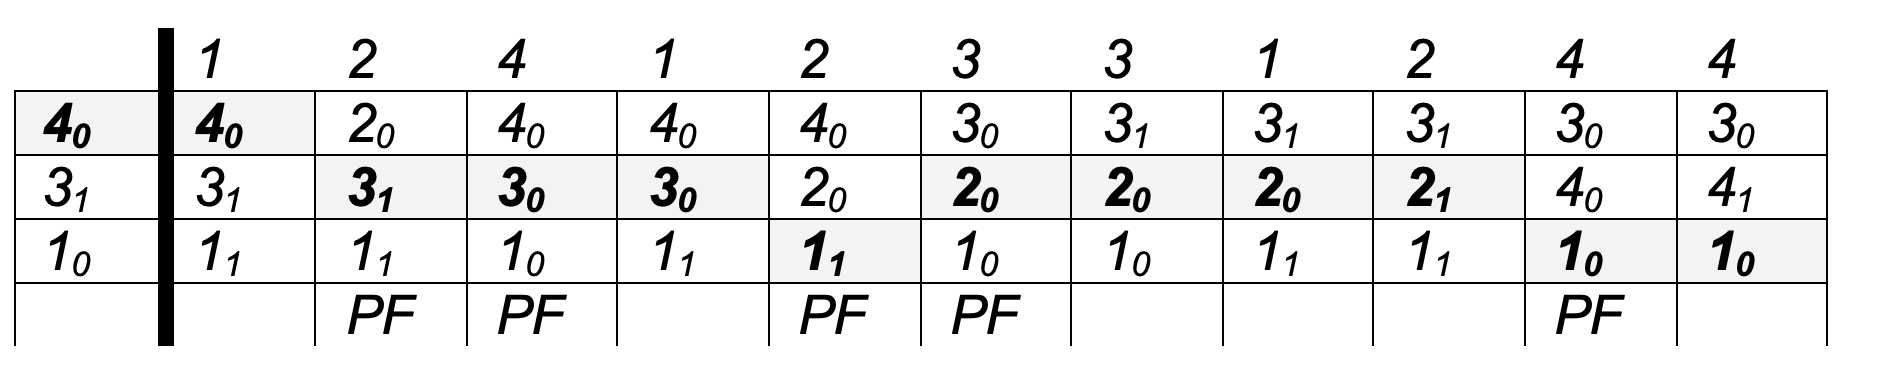
\includegraphics[width=0.8\textwidth]{images/ex04.png}
  \caption{Memory allocation}
\end{figure}

The total number of page faults is 5

\section{Exercise 5 - Page replacement}

Consider the following sequence of references in memory in the case of a program in which, for each access (addresses in hexadecimal, the Byte is addressed), it is indicated whether it is reading (R) or writing (W): R 3F5, R 364, W 4D3, W 47E, R 4C8, W 2D1, R 465, W 2A0, R 3BA, W 4E6, R 480, R 294, R 0B8, R 14E.

A. Assuming that both physical and logical addresses are on 12 bits, that paging with pages of 128 Byte is used, and that the maximum address the program can use is C10, compute how many pages are present in the address space of the program and calculate the internal fragmentation.

B. Determine the string of the page references (Switching from hexadecimal to binary is recommended to determine the page number correctly and, if necessary, the displacement/offset). An LRU (Least Recently Used) page replacement algorithm is used. Assume that 3 frames are available at physical addresses (expressed in hexadecimal) 780, A00, B00. The computation (after each access) of the resident set (the physical frames containing logical pages) is required.

C. Determine which and how many page faults (accesses to pages not present in the resident set) will occur.
Finally, tell which physical addresses the accesses are made to (among those listed above) R 3F5, W 4D3, R 3BA

\subsection{Solution}

A.

The total number of addressable pages (including those outside the proposed references) are C10 = 1100 0, 001 0000. The maximum page index 2*C (hexadecimal) = 2 * 12 (decimal) = 24 => In total, the addressable space includes 25 pages. Alternative method: C10H + 1 = 308910, NP = 3089 / 128 = 25

Internal fragmentation: The last page is occupied up to offset 0010000 (16) => fr. Int. = 128-17 = 111 Byte. Alternative: 128 - 3089% 128 = 128-17 = 111 (Byte)

B.

Logical addresses (p, d) (page, displacement). A page contains 128 Bytes, so 7 bits are needed for d, and 5 bits for p. References in binary: R (0011 1,111 0101), R (0011 0,110 0011), W (0100 1,101 0011). Reference string (you only need p, d is not needed): 7 (2 * 3 + 1), 6 (2 * 3 + 0), 9, 8, 9, 5, 8, 5, 7, 9, 9, 5, 1, 2 (note that p, given by the 5 most significant bits of the logical address, can be quickly calculated as the double of the first hexadecimal digit + the most significant bit of the second hexadecimal digit).

\begin{figure}[hbt]
  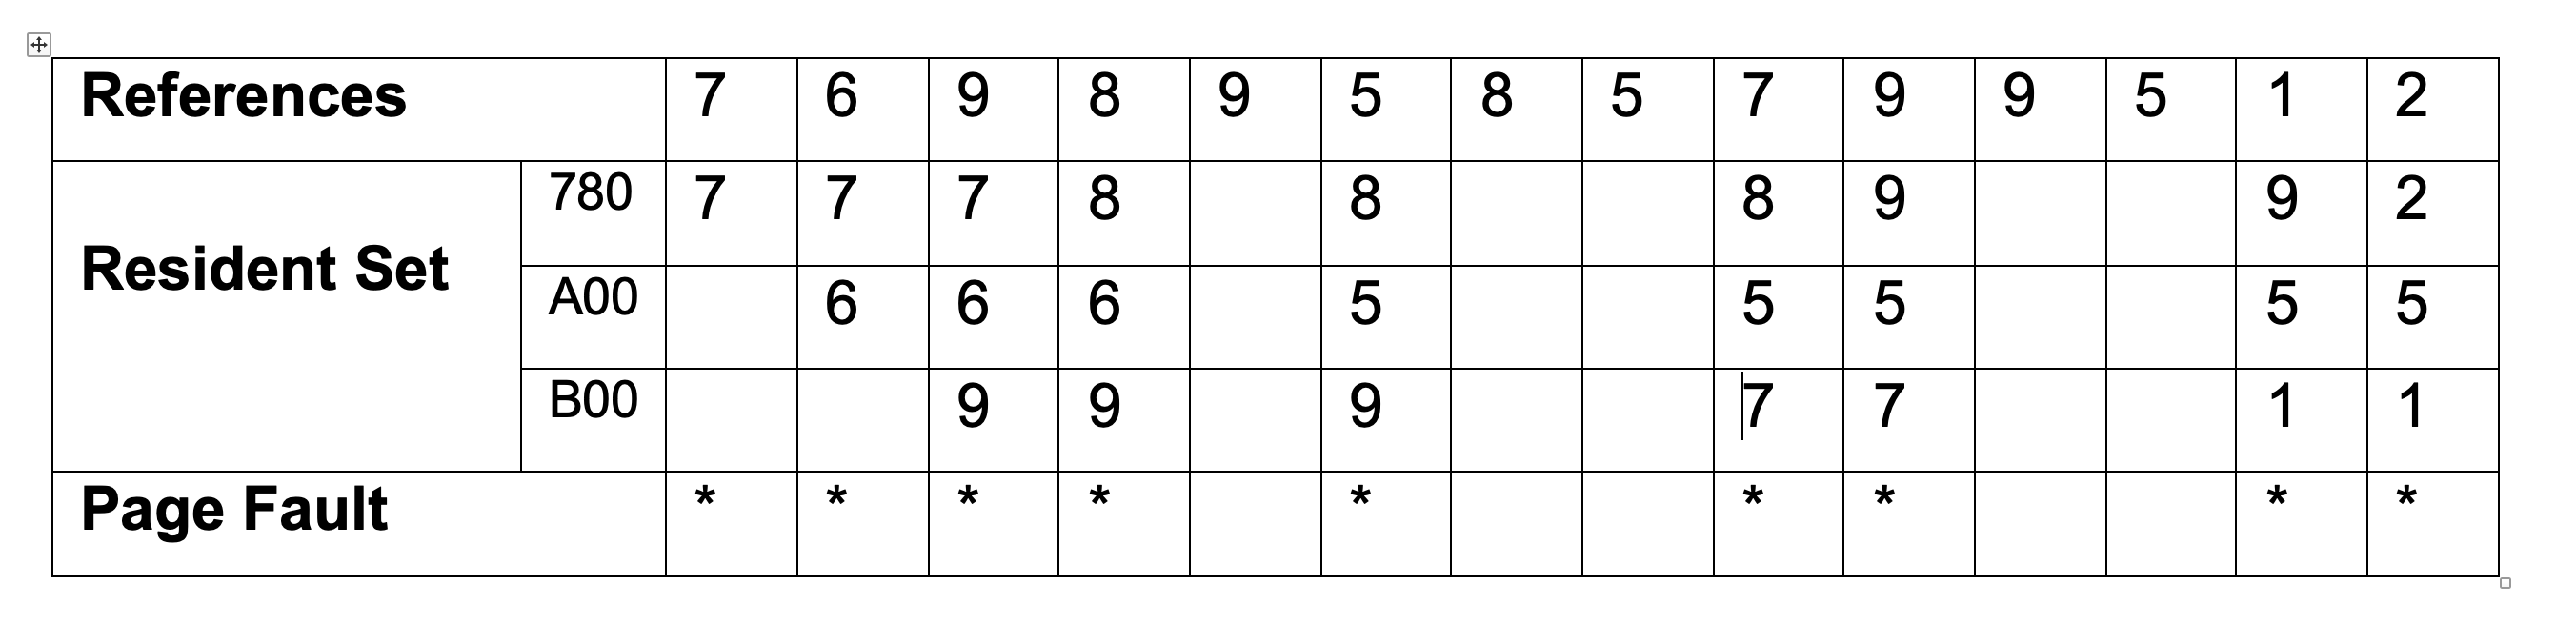
\includegraphics[width=0.8\textwidth]{images/ex05.png}
  \caption{Memory allocation}
\end{figure}

Total number of page faults: 9

Logical addr.:  R 3F5: (0011 1,111 0101)  W 4D3: (0100 1,101 0011) R 3BA: (0011 1, 011 1010)

Phisical addr.:  R  (0111 1,111 0101) = 7F5,  W (1011 0,101 0011) = B53,  R  (1011 0, 011 1010) = B3A

Warning: Logical page 7 is placed in two different frames in different moments. 



\section{Exercise 6 - Page replacement}

Consider the following sequence of references in memory in the case of a 4K word program in which, for each access (addresses in hexadecimal), it is indicated whether it is a read (R) or a write (W): W 3A1, R 3F5, R A64, W BD3, W 57E, R A08, R B85, W 3A0, R A1A, W A36, R B20, R 734, R AB8, R C4E, W B64.

Determine the string of page references, assuming their size is 512 words. An Enhanced Second-Chance page replacement algorithm is used. The modification bit (to be initialized to 0 at the first access to a new page after the relative page fault) is added to the reference bit (modify bit). Assume that a page is always modified in correspondence with a write, that 3 frames are available and that the algorithm operates with the following criterion: given the pointer to the current page (according to the FIFO strategy), a first turn is made , without changing the reference bit on the pages to locate the victim (the order of priority is (reference, modify): (0,0), (0,1), (1,0), (1,1)) ; once the victim has been determined, a second turn is made to reset the reference bits of the "saved" pages (between the starting position and the victim).

Determine which and how many page faults (accesses to pages not present in the resident set) will occur. The resident set is requested to be displayed (after each access), indicating the reference and modification bits for each frame. Number the pages starting from 0.

For this question, use the following scheme to carry out the exercise, indicating in the first line the string of references to pages (represented by choice in hexadecimal or decimal), in the second Read or Write, in the following three (representing the 3 frames of the resident set), the pages allocated in the corresponding frames, indicating the bits for each (reference, modify). Also indicate (by underlining, circling or placing an arrow) which page is at the top of the FIFO.
In the last line, indicate the presence or absence of a Page Fault.

\subsection{Solution}

Note that each hexadecimal digit represents 4 bits. Two digits are 8 bits. The division by 512 (29) is therefore obtained by eliminating the two least significant hexadecimal digits and further dividing by 2: in practice, the first of the 3 hexadecimal digits is divided by 2.

\begin{figure}[hbt]
  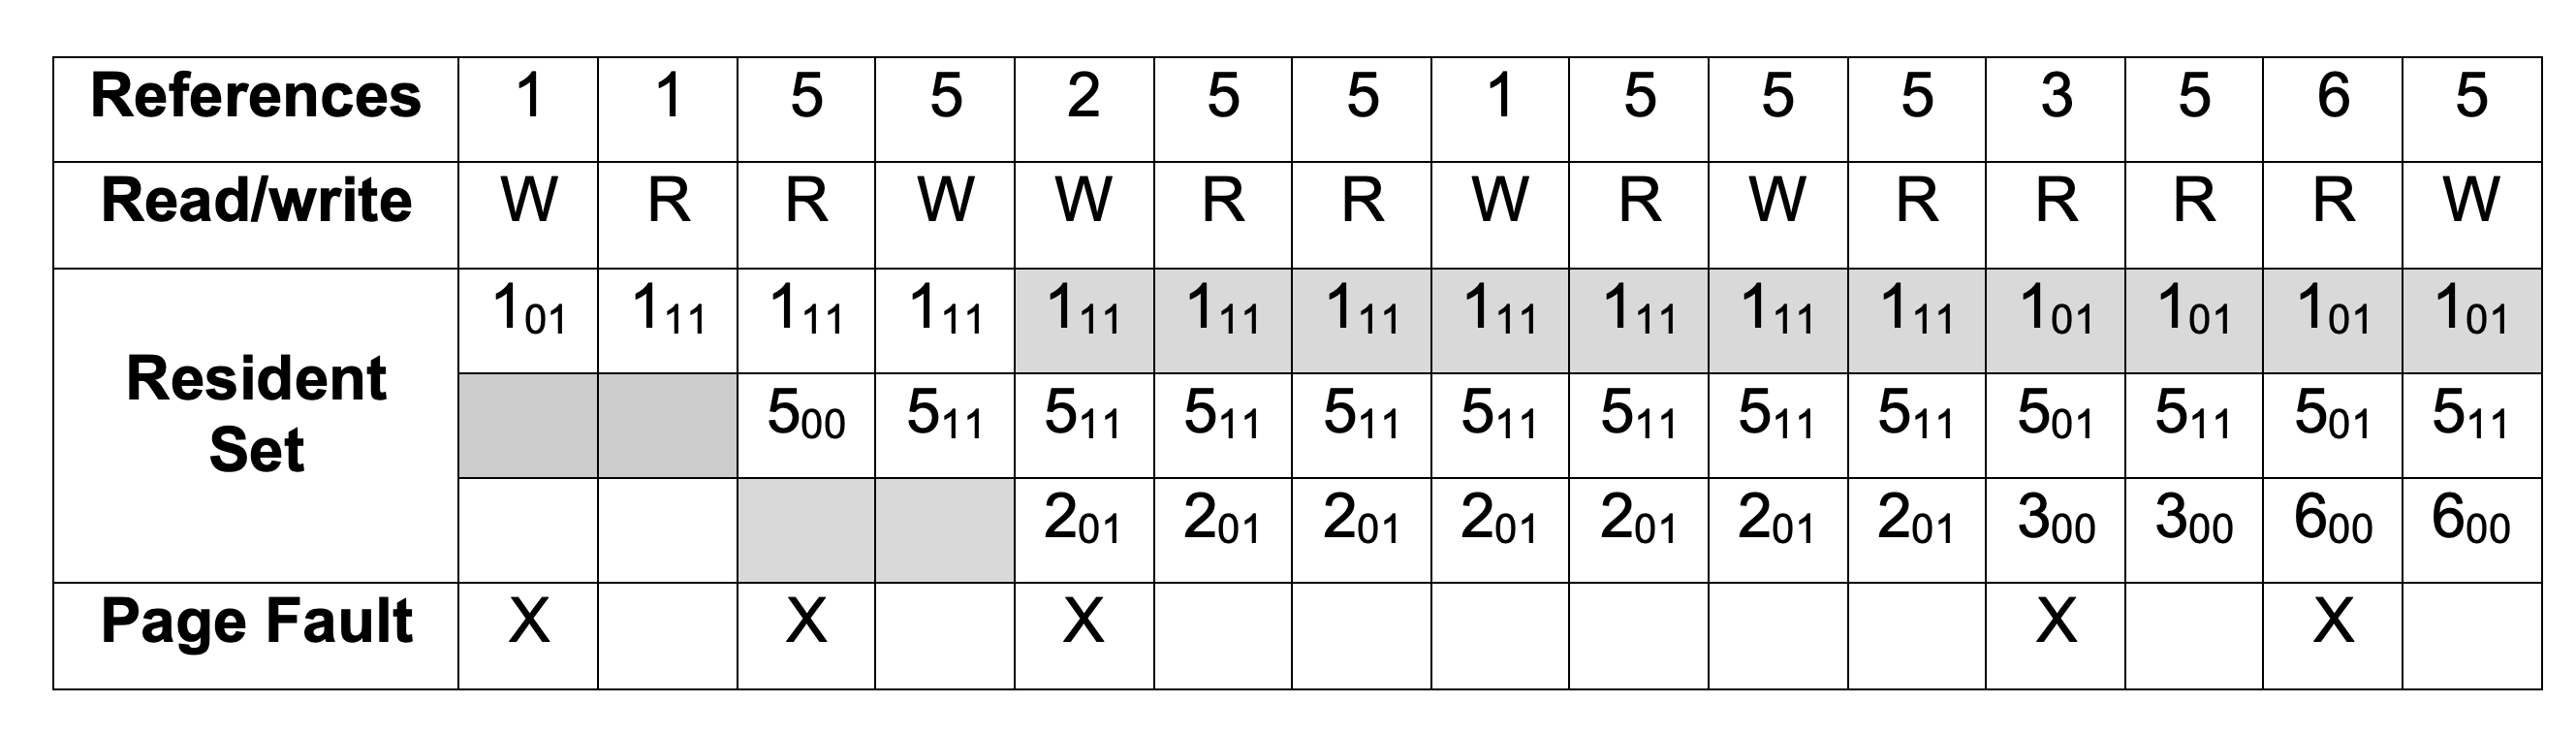
\includegraphics[width=0.8\textwidth]{images/ex06.png}
  \caption{Memory allocation}
\end{figure}

Total number of page faults: 5.

\section{Exercise 7 - Page replacement}


Consider the following sequence of references to pages in memory: 577517111434123.
Use a working-set page replacement algorithm (exact version) with window $\Delta$ = 3, assuming a maximum of 3 frames are available. Determine which and how many page faults (accesses to pages not present in the resident set) and page outs (removals of pages from the resident set) will occur. The resident set must be displayed (after each access).

We also want to define a measure of locality of the program carried out, based on the “Reuse Distance”. The Reuse Distance at time Ti (RDi), in which the page Pi is accessed, is defined as the number of pages (distinct and different from Pi) accessed starting from the previous access to Pi (assuming, conventionally, for the first access to a page, the total number of pages accessed up to that moment). For example, at time 3, in which the second access to page 5 is made, RD3 = 1, since between the two accesses to page 5 only one page was accessed twice (7). Given the various RDi, calculate the average RDavg value. The locality of the program carried out is defined as L = 1 / (1+ RDavg). Calculate the RDi, RDavg and L. 

For this question, use the following scheme to carry out the exercise. The references and the Reuse Distance at times 0 and 3 have already been indicated.

\subsection{Solution}

Note that a maximum of 3 frames are available, so the window $\Delta$ = 3 includes the current access at time Ti. The choice of the frame in the resident set is arbitrary. Therefore, other solutions are possible with permuted frames.

\begin{figure}[hbt]
  \centering
  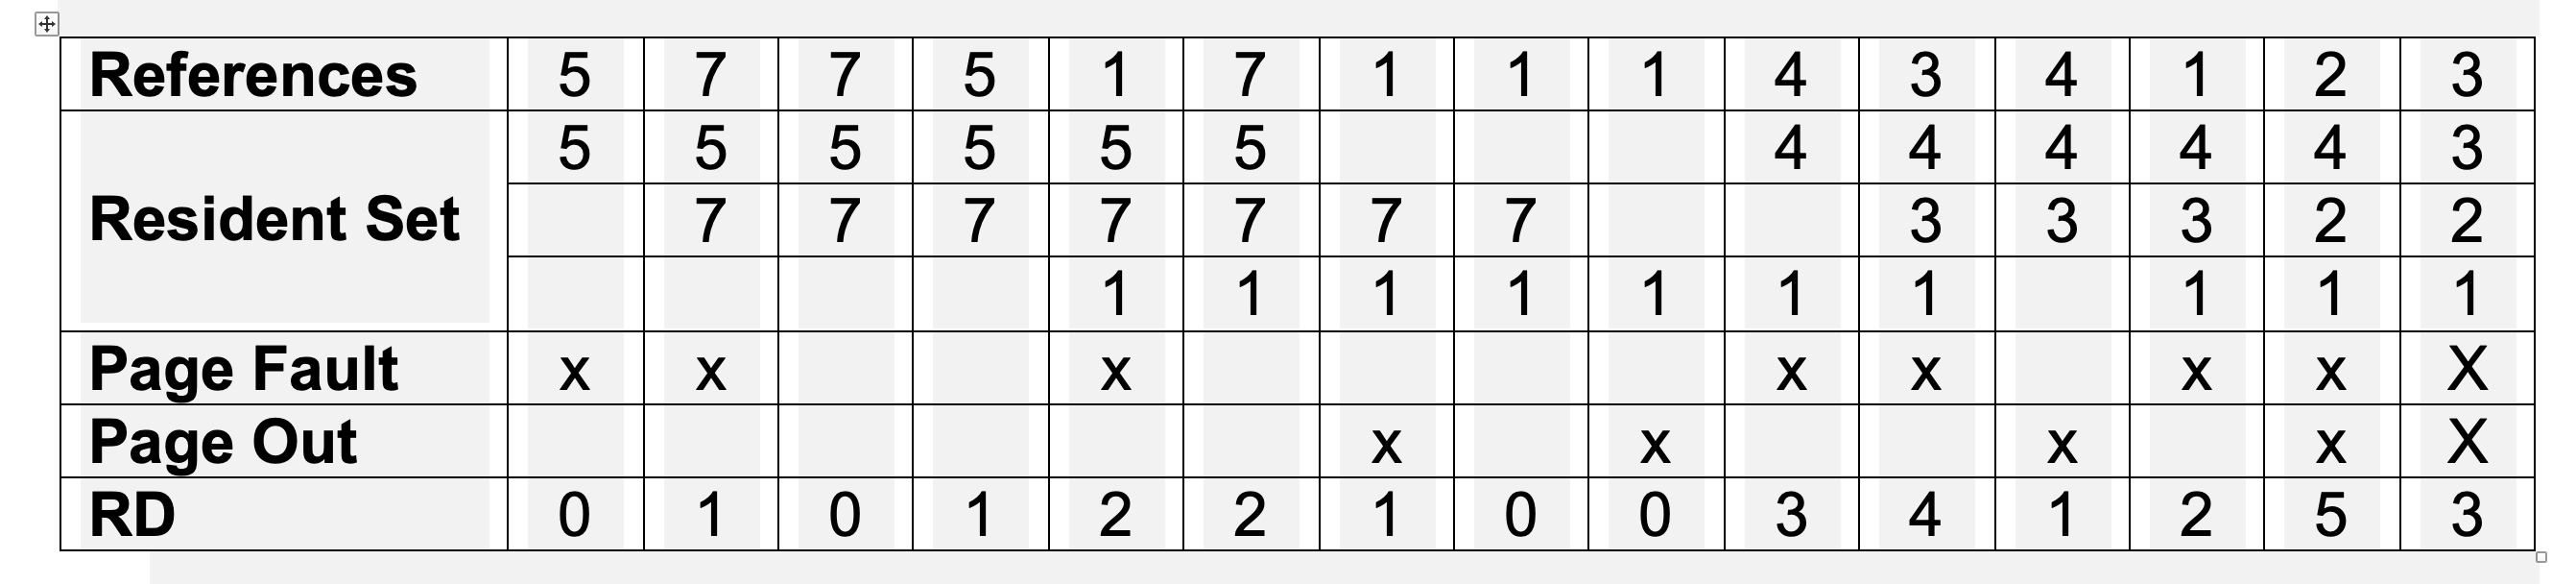
\includegraphics[width=0.8\textwidth]{images/ex07.png}
  \caption{Memory allocation}
\end{figure}

\#Page faults: 8 
\#Page out: 5	
RDavg: 25/15=5/3=1,67  	
L:  1/(1+5/3)=3/8=0,375 


\section{Exercise 8 - Page replacement}

Given the string of references to pages 3, 4, 1, (3, 1, 4, 4, 3, 1, 1) *10, where the syntax (...) *n indicates that the string in brackets is repeated/iterated n times (the string can, for example, derive from an iterative construct).

Use a working-set page replacement algorithm (exact version) with window $\Delta$ = 3. Suppose you call page-out the removal of a page from the resident set (as it leaves the working set). The references and the resident set are displayed in the following diagram after each reference, indicating the page faults (accesses to pages not present in the resident set) and the page-outs. Analyze the first two iterations of the substring repeated 10 times. 

ATTENTION: each row of the resident set represents a frame. Therefore a page present in a frame cannot change the row when it remains in the resident set. In the case of page fault without page-out, use the first free frame from above. In the case of page-out and (simultaneous) page-fault, the frame just freed (from page-out) is reused. If page-out and page-fault are related to the same page, the replacement algorithm takes them into account, avoiding both page-out and page-fault.

\subsection{Solution}

\begin{figure}[hbt]
  \centering
  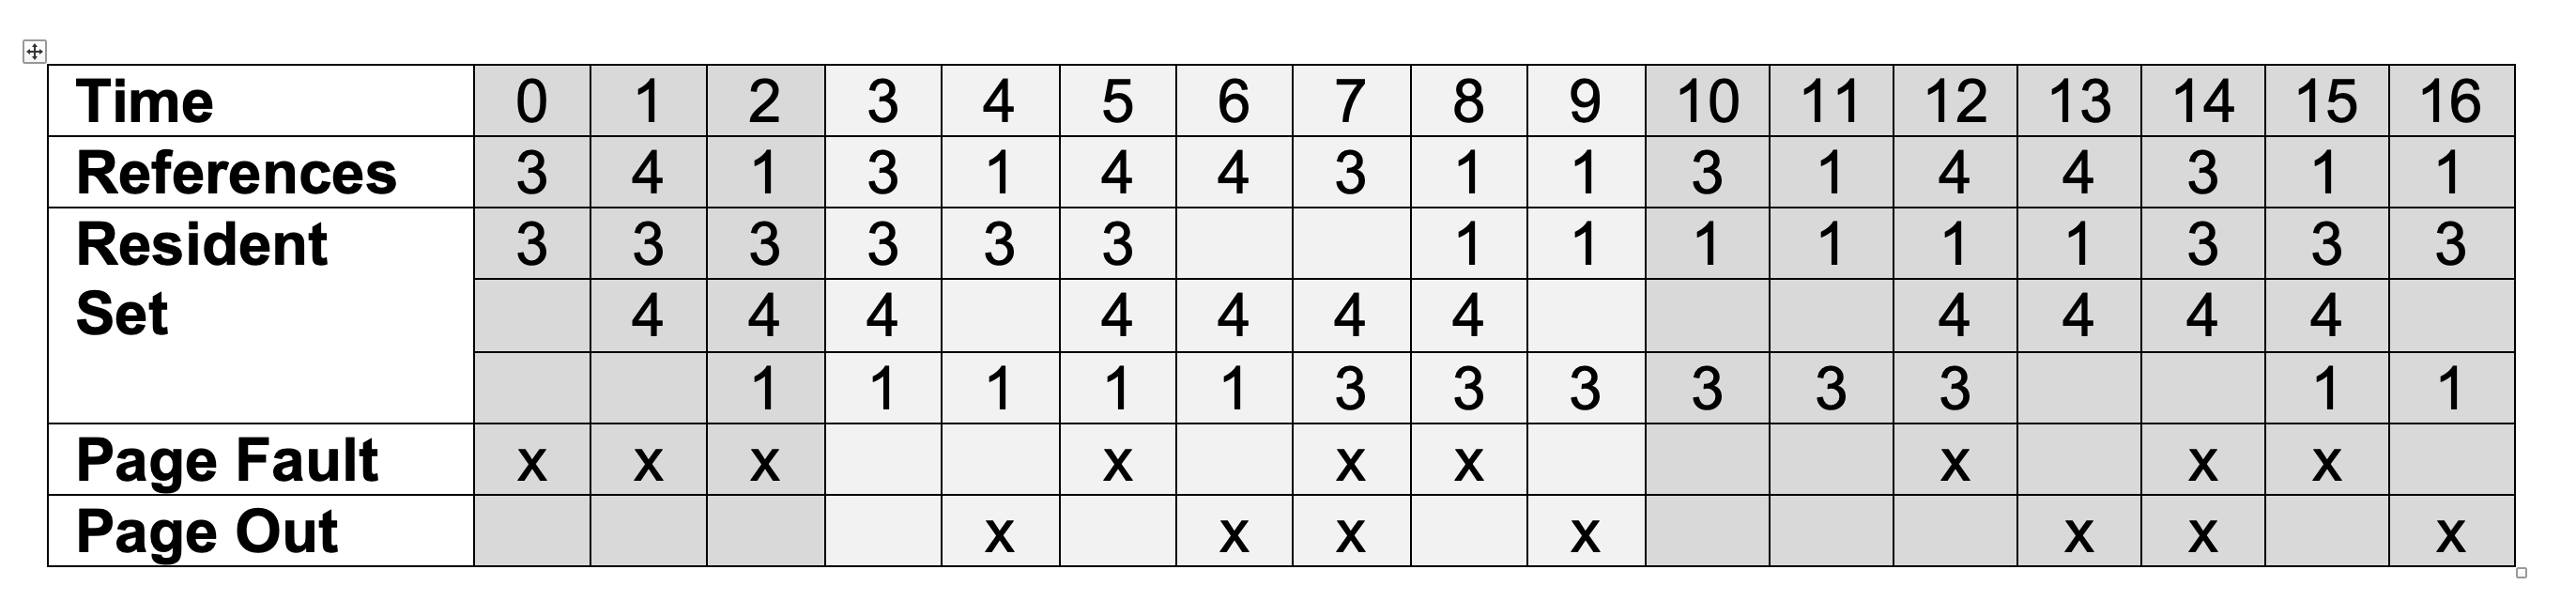
\includegraphics[width=0.8\textwidth]{images/ex08.png}
  \caption{Memory allocation}
\end{figure}

The behavior of the resident set in the 8 iterations not reported will be

\begin{itemize}
\item identical to that of the 10-16 interval (repeated 8 times)? (YES / NO motivate)
No, since, even if the period is 7 times, pages 1 and 3 are not in the same frame at the beginning and at the end of the period
\item or will it repeat the interval 3-16 4 times? (YES / NO motivate)
No, since although the 14 instants are the union of the first two periods of 7 instants, the first period has a different initial behavior due to the presence of page 4 at time 3 (the fourth)
\item or will it have a different configuration (which one?)?
The interval 3-16 is repeated 4 times, provided that page 4 is eliminated from time 3 and the page-out at time 4. Or (said in another way) the interval 10-16 is repeated 8 times, alternating at each iteration the contents of the first and third frames.
\end{itemize}

How many page faults and page-outs will there be in total (including the 8 missing iterations)?
9 PF and 7 PO in the displayed part, 8 * (3 PF and 3 PO) in the missing part: in total 33 PF and 31 PO



